\section{FPGA Implementation}\label{sec:fpga}

\subsection{Hardware overview}
The hardware consists of a preprocessor and a CNN core (\cref{fig:hardware-overview}). The preprocessor prepares the site crops and their neighbor values. Within the CNN core, an activation buffer stores the input crop and intermediate layer outputs. Input routing modules select and distribute the activations to an array of 100 multiply-accumulate (MAC) units. Weight and bias handlers supply the corresponding parameters from separate read-only memories (ROMs). The MAC results pass through requantization and, after the first two convolutional layers, max pooling. The layer output module arranges the results for the next layer or supplies the final two logits. A controller coordinates the memory reads, MAC operations, and progression through the six layers. Pipeline registers between these stages shorten the critical paths so that the design can run at a higher clock frequency.
\begin{sidewaysfigure}
    \centering
    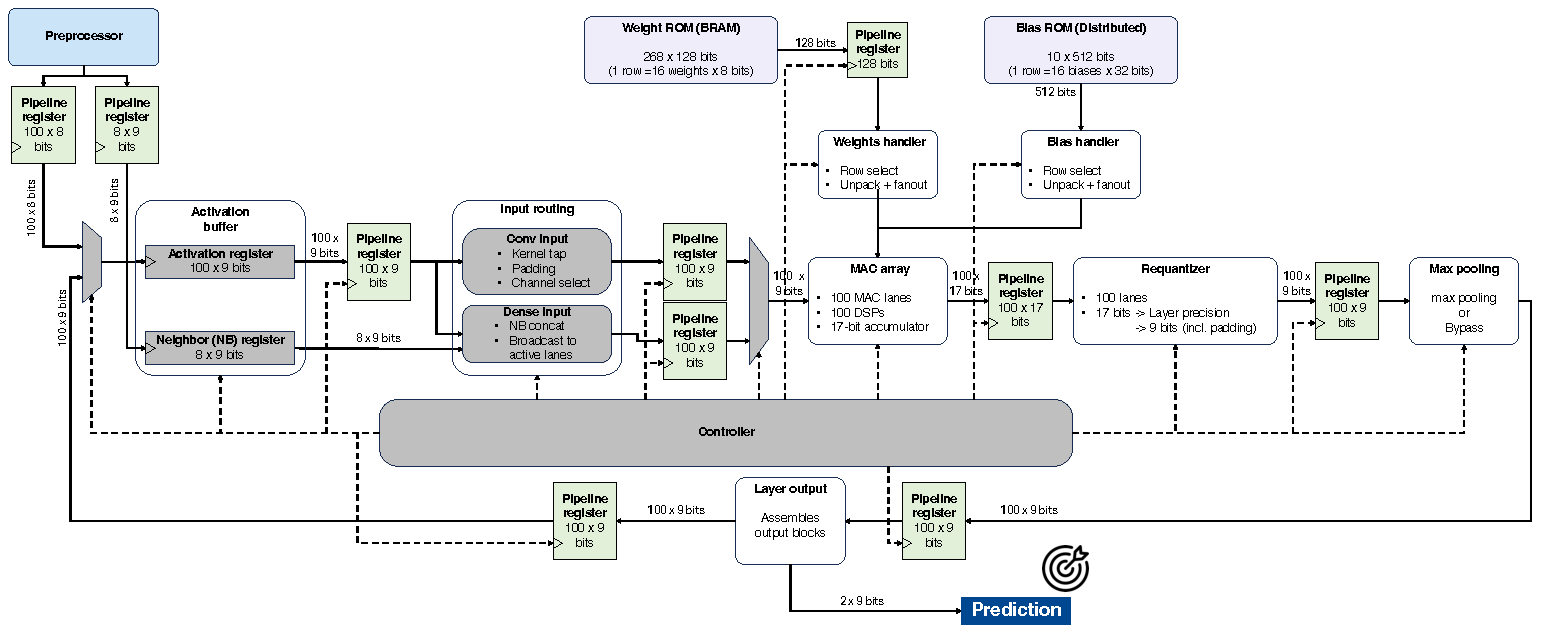
\includegraphics[width=\textheight]{hardware_overview_cropped.pdf}
    \caption{Hardware overview of the CNN core.}
    \label{fig:hardware-overview}
\end{sidewaysfigure}

\subsection{Preprocessing}
The preprocessor (\cref{fig:preprocessor}) converts a $28\times28$ frame into nine site inputs. Each input consists of a $10\times10$ crop and eight neighbor values. Crop extraction and normalization are performed incrementally as pixels arrive. After processing the entire frame, neighbor values are computed, and the site inputs are sequentially presented to the convolutional neural network (CNN).
\begin{figure}[tbp]
    \centering
    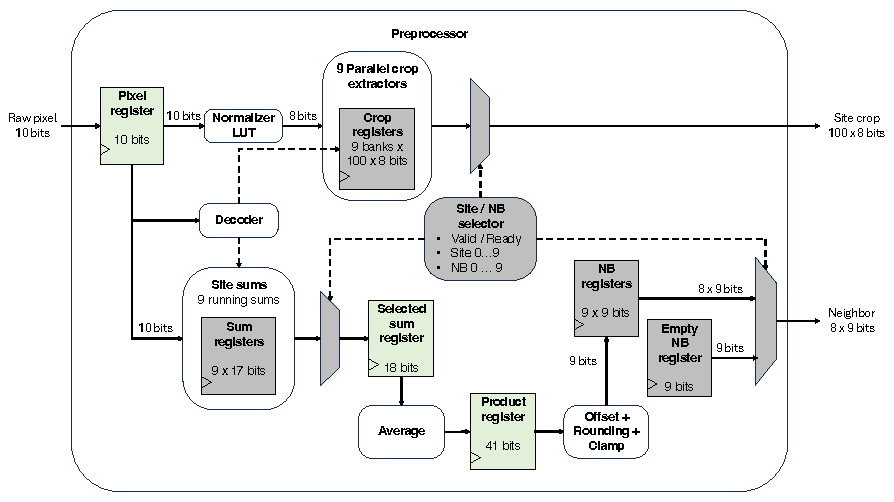
\includegraphics[width=0.95\textwidth]{preprocessing_cropped.pdf}
    \caption{Block diagram of the preprocessor.}
    \label{fig:preprocessor}
\end{figure}

\subsubsection{Pixel input and normalizer}
The input interface receives one unsigned 10-bit pixel per clock cycle when the valid signal is asserted. Pixels are delivered in row-major order, proceeding from left to right and top to bottom. Coordinate counters increment with each accepted pixel. Normalization is performed using the mean and scale parameters stored during training
\[
    p_{\mathrm{norm}} = \frac{p_{\mathrm{raw}}-\mu}{s}.
\]
The result for each valid raw pixel value is calculated before synthesis and stored in the \texttt{Normalizer} lookup table. Each raw pixel selects a signed 8-bit normalized value from this table.
\subsubsection{Crop extractors}
The positions of the nine sites are predetermined, resulting in constant starting coordinates for each crop. Nine parallel coordinate checks identify whether a pixel belongs to a given crop. For each matching crop, the pixel's local coordinates specify its position within the corresponding 100-element crop buffer. Each crop buffer contains 100 normalized 8-bit values, resulting in a total storage of 7200 bits across all nine buffers. Due to overlap between adjacent crops, a single incoming pixel may update multiple crop buffers simultaneously. Pixels that do not belong to any crop are discarded.
\subsubsection{Neighbor processor}
In parallel with crop extraction, nine running sums accumulate the raw pixel values associated with each crop. Each sum requires 17 bits, as the maximum sum of 100 unsigned 10-bit pixels is 102300. These sums are reset at the start of each new frame. Upon completion of pixel processing, each crop sum is converted into a neighbor feature. For a given sum $S_j$, the feature before quantization is defined as
\[
    n_j = \frac{S_j/100-\mu}{s\times s_{\mathrm{nb}}},
\]
Here, $s_{\mathrm{nb}}$ denotes the neighbor feature scale parameter stored during training. Consequently, the feature represents the normalized average brightness of the corresponding crop. The hardware implements division and scaling as a single constant multiplication, followed by subtraction of a constant offset. The multiplier applies the combined scaling, while the offset accounts for the stored mean. The result is rounded to the nearest value, with ties rounded to even, and saturated to the signed 9-bit neighbor format. A shared arithmetic unit sequentially processes the nine sums, and the resulting features are stored for later use across all sites. The selected sum is held in an 18-bit signed register, the 17-bit sum plus a sign bit, and its product with the 23-bit constant multiplier is 41 bits wide.
\subsubsection{Preprocessing controller}
A finite-state machine coordinates preprocessing through four states (\cref{fig:preprocessing-controller} in Appendix~\ref{app:preprocessing-controller}):
\begin{enumerate}
    \item \texttt{IDLE:} Accept incoming pixels, populate the crop buffers, and update the running sums. After pixel processing is complete, a start request begins neighbor conversion.
    \item \texttt{NEIGHBOR\_MULTIPLY:} Multiply the selected crop sum by the constant normalization factor.
    \item \texttt{NEIGHBOR\_FINISH:} Subtract the offset, round and saturate the result, and store the neighbor feature. Repeat the conversion for the next crop until all nine features are available.
    \item \texttt{PRESENT\_SITES:} Supply the selected crop and its eight neighbor features. Hold these values until the ready signal is asserted, then advance to the next site. After the ninth site is accepted, assert completion and return to \texttt{IDLE}.
\end{enumerate}


The output consists of an 800-bit crop vector and a 72-bit neighbor vector. A fixed neighbor index table selects the surrounding site features.

\subsection{Activation buffer}
The activation buffer stores the values required by the current CNN layer. It contains 100 signed 9-bit elements, forming a 900-bit vector. At the start of inference, this vector holds the normalized $10\times10$ site crop. As inference progresses, it is reused to store outputs from intermediate layers.
\subsubsection{Writing and reuse}
A multiplexer selects either the captured site crop or the completed output from the layer output module. The site scheduler first captures the crop and neighbor values in packet registers, then loads them into the CNN storage on the following clock edge.
Once an intermediate layer completes, its assembled output overwrites the previous contents. Values are stored consecutively according to the layout required by the next layer. For convolutional feature maps, spatial positions for each channel are grouped together, while dense layer features occupy the initial elements of the vector. If fewer than 100 elements are needed, the remaining positions are zero-filled. All values use a uniform 9-bit storage width, and values with lower signed precision are sign-extended.
\subsubsection{Reading}
The controller initiates a read operation before the input routing module selects activations for a multiply-accumulate (MAC) operation. The complete 100-element vector is read in parallel on a rising clock edge, accompanied by a valid signal. The input routing module subsequently selects the necessary spatial positions or dense input features. Because the buffer contains a complete vector, no address selection is required.
\subsubsection{Neighbor storage}
Eight signed 9-bit neighbor values are stored in a separate 72-bit register. These values are loaded simultaneously with the site crop and remain unchanged as intermediate layer outputs update the activation vector. The dense input module accesses these neighbor values during the second dense layer, where eight features from the previous layer are combined with the eight neighbor features.

\subsection{Input routing}
The input routing modules select the activations required for each MAC operation from the activation buffer. Separate modules handle convolutional and dense layers. A multiplexer selects the module's output according to the current layer.
\subsubsection{Convolutional input}
The convolutional input module receives the convolution index, input channel index, and kernel tap index from the controller. For each active MAC lane, a fixed spatial mapping selects the pixel corresponding to the current tap of the $3\times3$ kernel. Positions outside the feature map are assigned a value of zero, thereby implementing padding at the image boundaries. Different output channels use the same input pixels but different weights. The selected spatial values are repeated across the lanes assigned to those output channels.
The lane arrangement depends on the layer:
\begin{itemize}
    \item Conv0 processes one output channel with 100 spatial
          positions per block, using all 100 lanes.
    \item Conv1 processes four output channels with 25 spatial
          positions each per block, also using all 100 lanes.
    \item Conv2 processes 16 output channels with four spatial
          positions each, using 64 lanes.
\end{itemize}
Unused lanes in Conv2 are assigned a value of zero. The controller iterates through all input channels and kernel taps, and each MAC unit accumulates the contributions to its designated output. The next output blocks reuse the same routing configuration with a new set of weights.
\subsubsection{Dense input}
The dense input module selects one feature using the input feature index provided by the controller. This feature is broadcast to all active output lanes. Each lane receives a different weight and accumulates the result for one output neuron. The first dense layer selects from the 64 flattened outputs of Conv2 and uses eight output lanes. The second dense layer uses eight output lanes and selects from 16 inputs: eight features from the previous layer and eight neighbor values. Neighbor values are converted to the fixed-point format used by the dense input, with rounding and saturation. The final dense layer selects from 8 features and uses 2 lanes to compute the 2 logits. All inactive lanes are assigned a value of zero. In contrast to the convolutional input module, dense input routing does not require spatial mapping or kernel tap selection.

\subsection{MAC array}
A single array of 100 multiply-accumulate (MAC) units executes all three convolutional and three dense layers. The units operate in parallel, with each active lane computing a single output value (\cref{fig:mac-lane}). The controller reuses the array across output blocks, layers, and sites.
\begin{figure}[H]
    \centering
    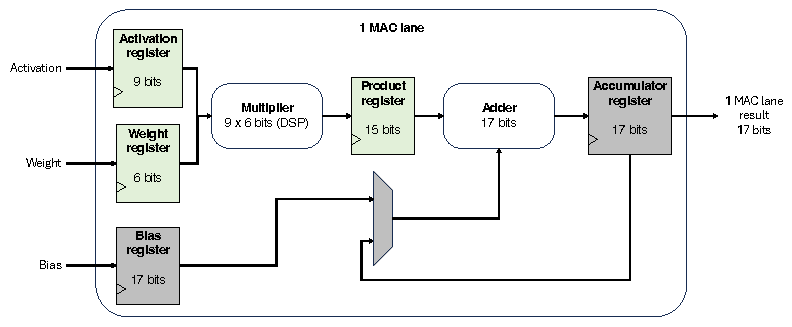
\includegraphics[width=0.8\textwidth]{mac_lane_cropped.pdf}
    \caption{One lane of the MAC array.}
    \label{fig:mac-lane}
\end{figure}

\subsubsection{Arithmetic}
Each lane receives a signed 9-bit activation and a signed 6-bit weight, the widest formats of \cref{tab:widths}. Layers with narrower formats are sign-extended to these widths. Their multiplication produces a signed 15-bit product, which is sign-extended before addition to a 17-bit accumulator. Both multiplication and accumulation are mapped to the FPGA's DSP blocks.
For an output value $y$, the array evaluates
\[
    y = b + \sum_{k=0}^{K-1} a_k w_k,
\]
where $b$ is the bias and $K$ is the number of contributions required for that output. Each valid MAC operation produces one activation-weight pair per lane.
\subsubsection{Bias initialization and accumulation}
During the first contribution to an output block, the controller asserts the bias-load signal and a multiplexer selects the bias as the addend.
\[
    b + a_0 w_0.
\]
For subsequent contributions, the multiplexer selects the previous accumulator value. Thus, bias initialization occurs simultaneously with the first product addition.
\subsubsection{Reuse across layers}
In convolutional layers, each lane accumulates contributions from all input channels and all nine kernel taps. Consequently, Conv0, Conv1, and Conv2 require 9, 36, and 72 products per output value, respectively.
In dense layers, each active lane represents one output neuron and accumulates over the input features. The three dense layers require 64, 16, and 8 products per output neuron,
respectively. Lanes outside the active output group receive zero activations and weights.
After the final contribution to a block, the controller waits until the MAC array has completed its pending operations. The finished accumulator values are then forwarded to the requantization module.

\subsection{Weight ROM and handler}

The weights of all six layers are stored in a synchronous ROM implemented in block RAM. The ROM contains 268 rows of 128 bits. Each row contains 16 signed 8-bit weight slots, with slot zero occupying the least significant bits. The stored weights fit the 6-bit precision used by the MAC array; the handler converts each slot to this width before distribution.

\subsubsection{Weight ROM architecture}
For convolutional layers, one row stores the weights for one input channel and one kernel tap across the output channels of the current block. The weights are shared across all spatial positions within the same output channel.
For dense layers, each row stores the weights connecting a single input feature to all output neurons. The number of rows assigned to each layer is listed in \cref{tab:weight-rows}.

\begin{table}[H]
    \centering
    \caption{Rows of the weight ROM for each layer.}
    \label{tab:weight-rows}
    \begin{tabular}{@{}lrr@{}}
        \toprule
        Layer & First row & Number of rows \\
        \midrule
        Conv0  &   0 & 36 \\
        Conv1  &  36 & 72 \\
        Conv2  & 108 & 72 \\
        Dense0 & 180 & 64 \\
        Dense1 & 244 & 16 \\
        Dense2 & 260 &  8 \\
        \bottomrule
    \end{tabular}
\end{table}

\subsubsection{Address selection}
The handler receives the layer, output block, input channel, and kernel tap indices from the controller and turns them into a row address. The row of a convolutional layer follows from its first row, the output block, the input channel, and the kernel tap, and the row of a dense layer from its first row and the input feature index. The row numbers are fixed constants in the design, so no multiplier is needed.

\subsubsection{Distribution to MAC lanes}
The handler unpacks the selected row and distributes its weights according to the layer's lane arrangement. Conv0 broadcasts a single weight across 100 spatial lanes. Conv1 broadcasts four weights to groups of 25 lanes. Conv2 broadcasts 16 weights to groups of four lanes. For Dense0 and Dense1, eight slots supply one weight to each active output lane. Dense2 uses two slots for its two output neurons. Unused lanes receive zero weights. A read-enable signal requests the ROM row. The row is read on a rising clock edge, and the accompanying valid signal indicates that the weights are available for the MAC operation.

\subsection{Bias ROM and handler}

The biases for all six layers are stored in a compact ROM implemented in distributed memory. This ROM consists of ten 512-bit rows, each divided into 16 signed 32-bit slots, with slot zero occupying the least significant bits. The bias handler retrieves the necessary slots and converts them to the 17-bit accumulator width.

\subsubsection{Bias ROM architecture}
Each convolutional output channel is assigned a single bias shared across all spatial positions, while each dense output neuron receives an individual bias. Consequently, a single ROM row contains all the biases required for a complete output block. The rows are arranged as listed in \cref{tab:bias-rows}.

\begin{table}[H]
    \centering
    \caption{Rows of the bias ROM for each layer.}
    \label{tab:bias-rows}
    \begin{tabular}{@{}lrrr@{}}
        \toprule
        Layer & First row & Number of rows & Used slots per row \\
        \midrule
        Conv0  & 0 & 4 &  1 \\
        Conv1  & 4 & 2 &  4 \\
        Conv2  & 6 & 1 & 16 \\
        Dense0 & 7 & 1 &  8 \\
        Dense1 & 8 & 1 &  8 \\
        Dense2 & 9 & 1 &  2 \\
        \bottomrule
    \end{tabular}
\end{table}

\subsubsection{Address selection}
The handler selects the row from the layer and output block indices supplied by the controller. Convolutional layers advance through their assigned rows as output blocks are processed, whereas each dense layer uses one fixed row.

\subsubsection{Distribution to MAC lanes}
In Conv0, a single bias is broadcast to all 100 spatial lanes. In Conv1, four biases are distributed to groups of 25 lanes each. In Conv2, 16 biases are assigned to groups of four lanes. For dense layers, each active output lane receives an individual bias, while unused lanes are assigned a value of zero. Both the ROM read and the handler's selection logic are combinational. The selected biases are supplied directly to the MAC array, which applies them with the first product addition of each output block. Each bias is therefore added once per output value, regardless of the number of input channels, kernel taps, or dense input features.

\subsection{Requantization}
The requantizer converts the completed MAC accumulators to the activation precision selected for each layer. All 100 lanes are processed in parallel by combinational logic between two pipeline registers. For each layer, a fixed right shift removes the fractional bits that the accumulator has in addition to the output format, that is, the difference $F_{\mathrm{acc}} - F_a$. The result is rounded to the nearest value, with ties rounded to even, and saturated to the representable range. ReLU sets negative values to zero in all layers except the final layer, whose signed outputs form the two logits. The results are sign-extended to the common 9-bit storage width.

\subsection{Max pooling}
Max pooling is performed after the first two convolutional layers. For each output channel, the largest value is selected within each non-overlapping $2\times2$ region, using a stride of two. This operation reduces the spatial dimensions from $10\times10$ to $5\times5$ after Conv0, and from $5\times5$ to $2\times2$ after Conv1. The final row and column of the $5\times5$ feature map are excluded, as they do not constitute complete pooling regions. Conv2 and the dense layers pass their values directly to the layer output module without pooling.

\subsection{Layer output assembly}

The layer output module combines the completed output blocks into the activation layout required by the next layer. The layer and output block indices determine where each block is placed in a 100-element buffer.
Conv0 produces four pooled blocks of 25 values, forming 100 activations. Conv1 produces two pooled blocks of 16 values, forming 32 activations. Conv2 supplies its 64 values in one block. Convolutional values are arranged consecutively by channel, so the Conv2 output also provides the flattened input to the first dense layer.
The first two dense layers each produce eight features, while the final layer produces two logits. Unused buffer elements are filled with zeros.
Once the final block of a layer has been assembled, the module asserts its output-valid signal. The controller then writes the completed vector to the activation buffer for the next layer. For the final layer, the two logits are supplied as the classification result, and the site is classified as occupied if the second logit is larger than the first.

\subsection{Site scheduler}
The site scheduler in \texttt{detector\_core} coordinates preprocessing and the sequential classification of the nine sites. It operates through five states (\cref{fig:site-scheduler} in Appendix~\ref{app:site-scheduler}):
\begin{enumerate}
    \item \texttt{IDLE:} Receive the frame pixels and wait for a start request after frame loading. The start request triggers neighbor feature conversion and advances the scheduler to the next state.
    \item \texttt{WAIT\_SITE:} Wait until the preprocessor presents a valid site packet. Accept the packet and capture its crop, eight neighbor values, and site index in registers. The 100 signed 8-bit crop values are sign-extended to the 9-bit activation width.
    \item \texttt{LOAD\_INPUT:} Load the captured crop into the activation buffer and the captured neighbor values into the separate neighbor register.
    \item \texttt{START\_INFERENCE:} Assert the CNN start signal, then advance to the result-waiting state.
    \item \texttt{WAIT\_RESULT:} Wait for the CNN result valid signal and present the site's logits and decision. Return to \texttt{WAIT\_SITE} for the next site, or assert the completion signal and return to \texttt{IDLE} after site eight.
\end{enumerate}


\subsection{CNN controller}
The controller coordinates the execution of all six layers for one site. A finite-state machine controls the activation and weight reads, MAC operations, and the transfer of completed layer outputs. Counters monitor the current layer, output block, input channel, or feature, and convolutional kernel tap. The controller operates through six distinct states (\cref{fig:cnn-controller} in Appendix~\ref{app:cnn-controller}):
\begin{enumerate}
    \item \texttt{IDLE:} Wait for a start request, then initialize the layer and operation counters.
    \item \texttt{READ\_ACTIVATION:} Request the activation vector from the activation buffer.
    \item \texttt{READ\_WEIGHTS:} Request the weight ROM row corresponding to the current operation.
    \item \texttt{MAC\_STATE:} Wait until both inputs are valid, then issue the MAC operation. The first operation of each output block also loads the biases.
    \item \texttt{EMIT\_BLOCK:} After the final contribution, wait until the MAC array finishes its pending operations, then release the completed accumulators for postprocessing.
    \item \texttt{WAIT\_LAYER\_OUTPUT:} After the final output block, wait for the layer output module to finish assembling the complete layer.
\end{enumerate}

Within convolutional layers, the controller iterates through nine kernel taps for each input channel. In dense layers, it processes input features in sequence. Completing an output block, the controller initiates the next block if further outputs are necessary. Upon finishing an intermediate layer, the controller enables writing to the activation buffer and proceeds to the next layer. After the final dense layer, it asserts the result valid and completion signals, then returns to the idle state.
